\section{Report Elements}
\label{sec:api_report_elements}

% Since characteristics use report elements, we introduce report elements first.
% Report elements were introduced in chapter \ref{chapter:xbrl}.
% There are multiple types of report elements, which are all represented by different classes in Brel.
% All of these classes implement a common interface called \texttt{IReportElement}.

% In total, we introduced six different types of report elements:

% \begin{enumerate}
%     \item \textbf{Concept} - Concepts define what kind of information a fact represents.
%     \item \textbf{Abstract} - Abstracts are used for grouping other report elements.
%     \item \textbf{Dimension} - Dimensions are used to describe a custom axis, along which a fact is positioned. 
%     \item \textbf{Member} - Members specify the point along a dimension that a fact is positioned at.
%     \item \textbf{LineItems} - Line items are used to group concepts into an axis, 
%     similar to how dimensions group members into an axis.
%     \item \textbf{Hypercube} - Hypercube elements describe a smaller sub-hypercube of the filing's global hypercube.
% \end{enumerate}

% Technically, only concepts, members and dimensions are part of the OIM, whereas the remaining three are not.
% However, from an editorial point of view, it makes sense to describe all of them in one place.
% Brel chooses to implement report elements as seen in figure \ref{fig:brel_report_element_classes}.

% \begin{figure}[H]
%     \centering
%     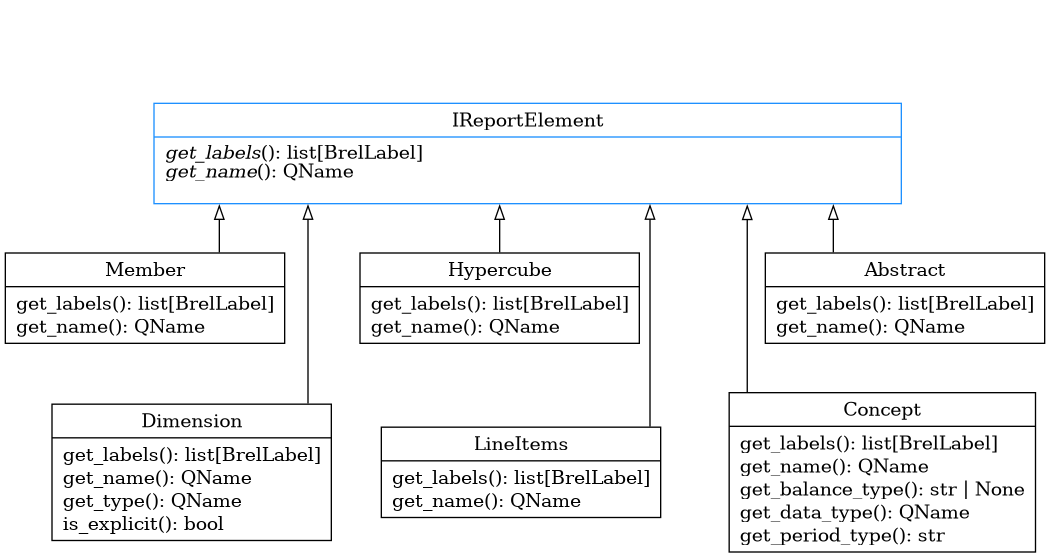
\includegraphics[width=\textwidth]{images/brel_report_elements_classes.png}
%     \caption{UML diagram of the report element classes in Brel}
%     \label{fig:brel_report_element_classes}
% \end{figure}

% As a general rule of thumb, we designed Brel's inheritance hierarchy to be as flat as possible.
% Since all report elements share a common interface, the next section covers the interface first.
% The subsequent sections then describe the different types of report elements.
Given that characteristics incorporate report elements, 
% we first discuss report elements.
we discuss report elements first.
They were introduced previously in chapter \ref{chapter:xbrl}.
Brel categorizes several types of report elements, each represented by distinct classes but unified under the \texttt{IReportElement} interface.
We categorize six principal types of report elements as follows:

\begin{enumerate}
\item \textbf{Concept} - Defines the nature of the information a fact represents.
\item \textbf{Abstract} - Utilized to group other report elements for organizational purposes.
\item \textbf{Dimension} - Describes a custom axis to position a fact within a specific context.
\item \textbf{Member} - Identifies a specific location along a dimension where a fact is positioned.
\item \textbf{LineItems} - Organizes concepts along an axis, analogous to the grouping function of dimensions for members.
\item \textbf{Hypercube} - Specifies a subset of the filing's global hypercube structure.
\end{enumerate}

From a technical standpoint, concepts, members, and dimensions directly relate to the OIM, while the rest do not.
Nevertheless, for clarity and coherence, all types are discussed collectively.
Brel's approach to implementing these elements is visualized in figure \ref{fig:brel_report_element_classes}, presenting a UML diagram of the report element classes.
Aiming for simplicity in Brel's design, the inheritance hierarchy is intentionally kept flat.
Following the introduction of the common interface, detailed discussions on each report element type are presented in subsequent sections.

\begin{figure}[H]
    \centering
    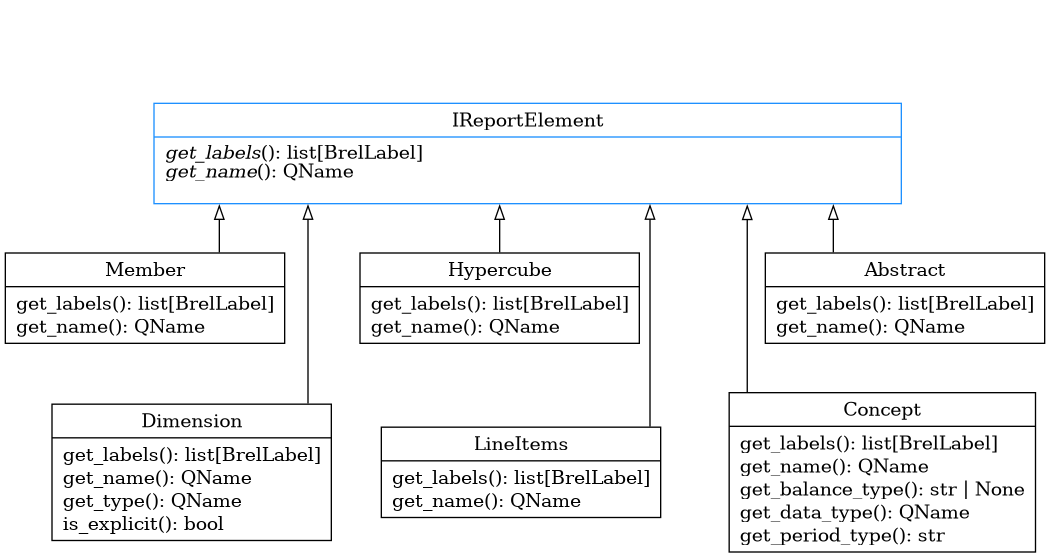
\includegraphics[width=\textwidth]{images/brel_report_elements_classes.png}
    \caption{UML diagram of the report element classes in Brel}
    \label{fig:brel_report_element_classes}
\end{figure}

\subsection{IReportElement}

The \texttt{IReportElement} interface defines the common interface that all report elements share.
In essence, a report element is a name which can be retrieved using the \texttt{get\_name} method.
% in this case a QName.

% Since QNames are not completely human-readable and do not support multiple languages,
% Brel also provides a method for getting the label of a report element.
% This chapter has not yet covered labels, but they will be described in section \ref{sec:labelLink}.
% However, they should be conceptually self-explanatory.
Given that QNames may not be entirely intuitive for human reading and lack multilingual support, 
Brel supplements this with a method to obtain a report element's label(s), 
although labels will be more thoroughly explained in section \ref{sec:labelLink}. 
A report element may have multiple labels, which can be retrieved using the \texttt{get\_labels} method.

\subsection{Concept}

The \texttt{Concept} element holds a central role within the XBRL framework, essential for every fact recorded. 
It specifies the nature of the data each fact represents.

Beyond the capabilities provided by the \texttt{IReportElement} interface,
the \texttt{Concept} also provides information about its associated facts.
% As mentioned in section \ref{sec:concepts}, concepts can constrain some characteristics of the facts that reference them.
As detailed in section \ref{sec:concepts}, concepts have the authority to impose restrictions on certain properties of the facts they are linked to.
The methods \texttt{get\_balance\_type}, \texttt{get\_data\_type} and \texttt{get\_period\_type} return the balance, 
data type and period type of the concept, respectively.

% The balance type is only available for monetary concepts, 
% and it indicates whether the concept represents an asset or a liability.
% They restrict the weights of calculation networks as described in section \ref{sec:calculationLink}.
% The data type of a concept indicates the data type of the value of the fact.
% The period type of a concept indicates the type of the period of the fact.
% It can be either "duration" or "instant".
The balance type applies solely to monetary concepts,
highlighting if the concept is categorized as an asset or a liability.
This classification influences the weighting within calculation networks, as outlined in section \ref{sec:calculationLink}.
A concept's data type specifies the value's data type for a given fact.
% Furthermore, a concept's period type delineates the temporal aspect of a fact,
Further, a concept's period dictates if a fact's period is a "duration" or an "instant".
% identifying it as either a "duration" or an "instant".

% \subsection{Dimension}

% Dimensions are used to describe a custom axis, along which a fact is positioned.
% Dimensions come in two different flavors, explicit and typed.
% Besides the methods that are inherited from the \texttt{IReportElement} interface,
% the \texttt{Dimension} has two additional methods.
% The first method \texttt{is\_explicit} returns a boolean value, indicating whether the dimension is explicit or not.
% The second method \texttt{get\_type} returns the type of the dimension, if it is typed.
% It raises an exception if the dimension is explicit.

% There is no need for the method \texttt{get\_members} in the \texttt{Dimension} class,
% since Brel models members differently.
% The dimension-member relationship is modeled as a parent-child relationship between the \texttt{Dimension} and \texttt{Member} objects in definition networks.
% So the members of a dimension change depending on the component that the dimension is part of.

% We chose to combine both typed and explicit dimensions into a single class,
% since they are semantically very similar.
% They occupy the same position within networks, but have some slight differences in their behavior.
% From a user's perspective, these differences are negligible.
\subsection{Dimension}

Dimensions define custom axes, along which facts are positioned.
There are two types of dimensions: explicit and typed.
In addition to inheriting methods from the \texttt{IReportElement} interface,
the \texttt{Dimension} class offers two specific methods.
The \texttt{is\_explicit} method returns a boolean indicating the nature of the dimension
%  — whether it is explicit.
as explicit or typed.
The \texttt{get\_type} method discloses the dimension's type for typed dimensions and triggers an exception for explicit ones.

% The \texttt{Dimension} class does not incorporate a \texttt{get\_members} method,
% as Brel adopts a distinct approach to modeling members.
% Instead, the dimension-member association is represented through a dimension-member link between \texttt{Dimension} and \texttt{Member} entities within definition networks,
% meaning the members associated with a dimension vary based on the component it is integrated with.

Merging typed and explicit dimensions into a singular class reflects their semantic alignment,
despite minor operational variances.
These differences are largely inconsequential from the user standpoint.
They also occupy the same position within networks, with only slight behavioral distinctions.

% \subsection{Abstract, Hypercube, LineItems, and Member}

% The \texttt{Abstract}, \texttt{Hypercube}, \texttt{LineItems} and \texttt{Member} classes are all very similar.
% Essentially, their only differentiating factor is their name.
% Besides that, they all provide the same methods and attributes.
% Namely, they implement the \texttt{IReportElement} interface.
% We decided to split them into four different classes, since they are semantically different.

\subsection{Abstract, Hypercube, LineItems, and Member}

The classes \texttt{Abstract}, \texttt{Hypercube}, \texttt{LineItems}, and \texttt{Member} bear a strong resemblance to each other.
% with their names serving as the primary distinction.
Aside from their names, they offer identical functionalities and properties.
The decision to segregate them into separate classes is based on their distinct semantic roles,
despite their functional similarities.
